\section{Trafiktællinger}
\label{sub:trafiktaellinger}
Dette afsnit tager udgangspunkt i kilden:
\\ http://vej08.vd.dk/mastra/mastradok/dok/TrafiktaellingerPlanUdfoerEfterb.pdf

Trafiktællinger udføres til mange formål. Det gælder alt fra at kontrollere den overordnede vejplanlægning til at undersøge klagesager om for høje trafik hastigheder. Trafiktællinger bruges bl.a. til at finde løsninger til opgaver omhandlende trafiksikkerhed, kapacitet og miljøforhold, samt statistikker over trafikudviklingen og hastigheden af vejnettet. Man kan foretager trafiktællinger manuelt eller ved brug af maskiner. 
Manuelle tællinger fungerer ved at personer registrere trafikken på det pågældende sted, ofte ved hjælp af tælleblokke, håndtællere eller håndterminaler. Ved maskine tælling fortages registreringerne automatisk ved brug af et tælleapparat, hvor mennesker ikke medvirker.

\subsection{Manuel tælling}
\label{sub:manuel_taelling}
Manuel tælling er som sagt, hvor det er mennesker der tæller trafikken. Manuel tælling er en god metode, når der ønskes at kende trafikkens specifikke trafikstrømme. Et typisk forløb for manuel tælling er opbygget af 6 trin.
\\\\
1) Som det første skal formålet for tællingen bestemmes, samt hvilken resultat type, som ønskes af opnå.
\\\\
Vores formål med trafiktællingen er tælle hvor mange fodgængere, cykelister og billister som befinder sig inde ved Nytorv og Østerågade. Hvorefter vi vil omregne resultaterne til årsdøgnstrafik ÅDT. Desuden vil vi notere, hvilken retning trafikanten kom fra og hvilken retning trafikanten skal hen, og herved kunne lave et flowkort af trafikken.
\\\\
2) Der skal besluttes placeringen af tælleposterne, hvor der skal tages hensyn til at tælleren ikke genere trafikken. Tællerne skal også have frit udsyn for parkerende biler, buskaser og lignende under hele tælleperioden. Man skal derfor overveje om forholdene kan ændre sig undervejs.For at have et optimalt overblik over tælleområdet, vurderede vi på tælledagen hvor vi bedst kunne placere os uden at generer trafikken og noterer alle trafikanterne. Vi endte med at sidde uden for The Harp som ligger lige ud til Østerågade og på første sal i McDonald’s hvor der var godt overblik af Østerågade og Nytorv.
\\\\
3) En af de betydelige usikkerheder ved trafiktællinger, er valget af tælleperioden. Der kan være meget stor variation fra dag til dag og time til time, hvis man. ønsker at finde årsdøgntrafikken. Der er f.eks. stor forskel på trafikmængden i weekenden kontra hverdage og myldertiden om morgen og eftermiddagen kontra midt på dagen og om aftenen og natten. Manuelle tællinger vare typisk 4, 6 eller 12 timer og sjældent et helt døgn. Vi valgte at lave trafiktællingerne tirsdag d. 24 november kl. 13:00 til 15:00. Vi havde valgt tidspunktet ud fra hvornår vi havde tid i forhold til vores skema, og vi vurderede at det er omkring dette tidspunkt på dagen hvor der er flest mennesker i området, eftersom at der ligger mange butikker i nærheden.
\\\\
4) Når tælleposterne og tidspunkterne er fastlagt, bestemmes antallet af tællere til posterne, efter trafikmængden ved stedet. Ifølge vejdirektoratet er kvaliteten af resultaterne afhænger af antal tællere. Er tælleposterne underbemandet, vil resultaterne blive uanvendelige. Hvis man er uvidende om trafikmængden, og dermed antallet af tæller som er nødvendige, kan man foretage en prøvetælling inden.

\begin{figure}[htbp]
   \label{fig:taellingstype}
   \centering
   \begin{adjustbox}{max width=\textwidth}
     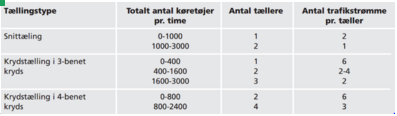
\includegraphics[scale=1]{billederogfigur/taellingstype.jpg}
  \end{adjustbox}
   \caption{Tællingstyper}
 \end{figure}
 
 \begin{figure}[htbp]
   \label{fig:krydstaelling}
   \centering
   \begin{adjustbox}{max width=\textwidth}
     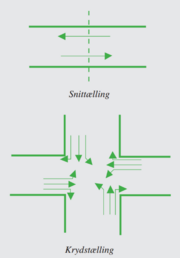
\includegraphics[scale=1]{billederogfigur/krydstaelling.jpg}
  \end{adjustbox}
   \caption{Skitse af krydstælling}
 \end{figure}
 
Der skal også bestemmes valget af tælleudstyr. Ved mindre trafikmængder kan der anvendes blyant og papir, ved stører trafikmængder anvendes ofte håndtællere, håndterminaler eller tællepulte. Da der er mange trafikanter i området og vi alle er uerfarne med trafiktællinger, har vi valgt at vi alle 6 i gruppen skal ud og tælle. Vi har valgt at lave et tælleskema i Excel, som vi printer ud i papir og kan afkrydse vores talte trafikanter i.
\\\\
5) Inden tællerne begynder, er det vigtigt at de er sat sig ind i overstående bestemmelser for tælleforløbet, således der ikke opstår tvivler undervejs. Ligeledes udarbejdes et tælleskema inden tællingen påbegyndes. 
\\\\
6) Resultatbehandling af tællingen. 
Der skal også bestemmes valget af tælleudstyr. Ved mindre trafikmængder kan der anvendes blyant og papir, ved stører trafikmængder anvendes ofte håndtællere, håndterminaler eller tællepulte.
Da der er mange trafikanter i området og vi alle er uerfarne med trafiktællinger, har vi valgt at vi alle 6 i gruppen skal ud og tælle. Vi har valgt at lave et tælleskema i Excel, som vi printer ud i papir og kan afkrydse vores talte trafikanter i.
 
\begin{figure}[htbp]
   \label{fig:trafiktaellingen}
   \centering
   \begin{adjustbox}{max width=\textwidth}
     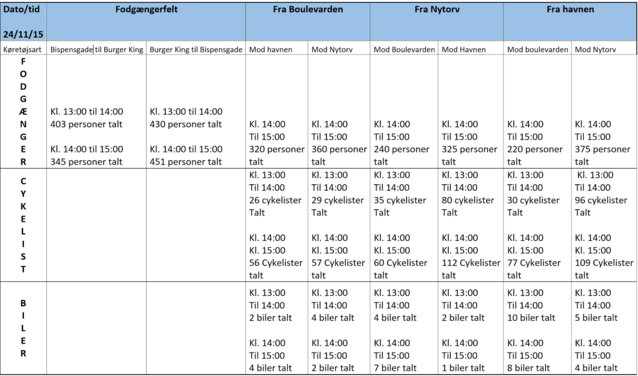
\includegraphics[scale=1]{billederogfigur/trafiktaellingen.jpg}
  \end{adjustbox}
   \caption{Resultat af trafiktælling}
 \end{figure}
Der findes ingen omregningsfaktor af fodgængere til ÅDT, derfor har vi vurderet vores tælling, ud fra forholdende på tælledagen. Vi noterede 2636 fodgængere tirsdag den 24 november Kl. 14:00 til 15:00. På dette tidspunkt har skole og gymnasieelever måske fået fri, mens alle som har et 8 til 16 job stadig er på arbejde. Derfor ville der måske være flere hvis tællingen var taget senere. Til gengæld hvis tællingerne var taget tidligere og midt i skoletiden ville antallet af fodgængere nok være mindre. En anden faktor er, at det regnede mens vi talte. Vi tror at regnvejret vil holde mange indendørs og vente til en anden dag med at shoppe i midtbyen. Desuden har dagen og årstiden en stor indflydelse på antallet af fodgængere på Nytorv og Østerågade. Eftersom at der er mange butikker i området, er det ikke bolig – arbejde trafik som kommer her. Det er nærmere folk, med et ærinde som f.eks. at shoppe eller at gå på café. Derfor kunne man forestille sig at der vil komme flere mennesker i weekenden hvor folk har fri for arbejde end i hverdagen. I sommerferien vil man også kunne finde meget mere liv, fordi folk mødes, og der bliver afholdt diverse arrangementer nede i byen. Hvis vi skal konkludere på usikkerhederne, er antallet af fodgængere i Østerågade og Nytorv meget situations afhængig. Det vil være stor forskel på en varm dag i sommerferien hvor byen tiltrækker med faciliteter og arrangementer og en kold regnvejrsdag i efteråret.

\subsection{Opregning af trafiktællinger til ÅDT}
\label{sub:opregning}
Ved at opregne et antal talte cykler og biler på én dag til ÅDT, vil der altid være en usikkerhed. 
I følgende resultatbehandling vil der være fokus på en trafiktælling af cykler og biler ved Nytorv i Aalborg tirsdag d. 24/11 i tidsrummet 14-18. I dette tidsrum er der tale om en blanding af såkaldt bolig/arbejde og by/lokal trafik, da det er i dette tidspunkt, at gennemsnittet af befolkningen får fri fra arbejde og skole, går på indkøb, og i dette tidsrum, at folk skal hjem til sig selv.
Antallet af biler, som vi fik talt i perioden var 104, og antallet af cykler i samme periode var 1408.
For at opregne en trafiktælling, som denne til årsdøgnstrafik, skal man bruge en bestemt formel:
$$ T \times FDT \times FUHDT \times FUDT \times FÅDT = ÅDT $$ eller $$ UDT \times FÅDT = ÅDT$$ , hvor:

$$T = Talt trafik$$

$$UDT = Ugedøgstrafik$$

$$FDT = Opregningsfaktor til døgntrafik i tælleugen$$

$$FUHDT = Opregningsfaktor til ugehverdagsdøgntrafik i tælleugen$$

$$FUDT = Opregningsfaktor til ugedøgntrafik i tælleugen$$

$$FÅDT = Opregningsfaktor til årsdøgntrafik i tælleåret$$ 

$$FÅR = Opregningsfaktor fra tælleår til andet år$$

Tallene aflæses i skemaerne på side 102-117. Den sidstnævnte formel til at udregne ÅDT’en, er den mest oplagte, da der findes en nem metode at finde frem til UDT, og hernæst skal FÅDT blot aflæses og ganges med UDT, for at vi kan finde ÅDT.

\subsection{ÅDT}
\label{AEDT}
\subsubsection{Cyklernes samlede ÅDT på Nytorv i Aalborg}
$$DT = T \times FDT = 1408 \times 1/(0,083+0,106+0,098+0,065) = 4.000$$
$$UHDT = DT \times FUHDT = 4.000 \times 0,95 = 3.800$$
$$UDT = UHDT \times FUDT = 3.800 \times 0,81 = 3.078$$
$$ÅDT = UDT \times FÅDT = 3.078 \times 1,15 = 3.540$$
\subsubsection{ÅDT for cykler fra Boulevarden mod Havnen}
$$DT = T \times FDT = 162 \times 1/(0,083+0,106+0,098+0,065) = 460 $$
$$UHDT = DT \times FUHDT = 460 \times 0,95 = 437$$
$$UDT = UHDT \times FUDT = 437 \times 0,81 = 354$$
$$ÅDT = UDT \times FÅDT = 354 \times 1,15 = 407$$
\subsubsection{ÅDT for cykler fra Boulevarden mod Nytorv}
$$DT = T \times FDT = 172 \times 1/(0,083+0,106+0,098+0,065) = 489$$
$$UHDT = DT \times FUHDT = 489 \times 0,95 = 465$$
$$UDT = UHDT \times FUDT = 465 \times 0,81 = 377$$
$$ÅDT = UDT \times FÅDT = 377 \times 1,15 = 434$$
\subsubsection{ÅDT for cykler fra Nytorv mod Boulevarden}
$$DT = T \times FDT = 176 \times 1/(0,083+0,106+0,098+0,065) = 500$$
$$UHDT = DT \times FUHDT = 500 \times 0,95 = 475$$
$$UDT = UHDT \times FUDT = 475 \times 0,81 = 385$$
$$ÅDT = UDT \times FÅDT = 385 \times 1,15 = 443$$
\subsubsection{ÅDT for cykler fra Nytorv mod Nytorv}
$$DT = T \times FDT = 286 \times 1/(0,083+0,106+0,098+0,065) = 813$$
$$UHDT = DT \times FUHDT = 813 \times 0,95 = 772$$
$$UDT = UHDT \times FUDT = 772 \times 0,81 = 625$$
$$ÅDT = UDT \times FÅDT = 625 \times 1,15 = 719$$
\subsubsection{ÅDT for cykler fra Havnen mod Boulevarden}
$$DT = T \times FDT = 224 \times 1/(0,083+0,106+0,098+0,065) = 636$$
$$UHDT = DT \times FUHDT = 636 \times 0,95 = 604$$
$$UDT = UHDT \times FUDT = 604 \times 0,81 = 489$$
$$ÅDT = UDT \times FÅDT = 489 \times 1,15 = 562$$
\subsubsection{ÅDT for cykler fra Havnen mod Nytorv}
$$DT = T \times FDT = 388 \times 1/(0,083+0,106+0,098+0,065) = 1.102$$
$$UHDT = DT \times FUHDT = 1.102 \times 0,95 = 1.047$$
$$UDT = UHDT \times FUDT = 1.047 \times 0,81 = 848$$ 
$$ÅDT = UDT \times FÅDT = 848 \times 1,15 = 975$$
\subsubsection{Bilernes samlede ÅDT på Nytorv i Aalborg}
$$DT = T \times FDT = 216 \times 1/(0,068+0,091+0,095+0,073) = 661$$
$$UHDT = DT \times FUHDT = 661 \times 1,02 = 674$$
$$UDT = UHDT \times FUDT = 674 \times 0,91 = 613$$
$$ÅDT = UDT \times FÅDT = 613 \times 1,00 = 613$$
\subsubsection{ÅDT for biler fra Boulevarden mod Havnen}
$$DT = T \times FDT = 24 \times 1/(0,068+0,091+0,095+0,073) = 73$$
$$UHDT = DT \times FUHDT = 73 \times 1,02 = 74$$
$$UDT = UHDT \times FUDT = 74 \times 0,91 = 67$$
$$ÅDT = UDT \times FÅDT = 67 \times 1,00 = 67$$
\subsubsection{ÅDT for biler fra Boulevarden mod Nytorv}
$$DT = T \times FDT = 24 \times 1/(0,068+0,091+0,095+0,073) = 73$$
$$UHDT = DT \times FUHDT = 73 \times 1,02 = 74$$
$$UDT = UHDT \times FUDT = 74 \times 0,91 = 67$$
$$ÅDT = UDT \times FÅDT = 67 \times 1,00 = 67$$
\subsubsection{ÅDT for biler fra Nytorv mod Boulevarden}
$$DT = T \times FDT = 44 \times 1/(0,068+0,091+0,095+0,073) = 135$$
$$UHDT = DT \times FUHDT = 135 \times 1,02 = 138$$
$$UDT = UHDT \times FUDT = 138 \times 0,91 = 126$$
$$ÅDT = UDT \times FÅDT = 126 \times 1,00 = 126$$
\subsubsection{ÅDT for biler fra Nytorv mod Havnen}
$$DT = T \times FDT = 12 \times* 1/(0,068+0,091+0,095+0,073) = 37$$
$$UHDT = DT \times FUHDT = 37 \times 1,02 = 38$$
$$UDT = UHDT \times FUDT = 38 \times 0,91 = 35$$
$$ÅDT = UDT \times FÅDT = 35 \times 1,00 = 35$$
\subsubsection{ÅDT for biler fra Havnen mod Boulevarden}
$$DT = T \times FDT = 76 \times 1/(0,068+0,091+0,095+0,073) = 232$$
$$UHDT = DT \times FUHDT = 232 \times 1,02 = 237$$
$$UDT = UHDT \times FUDT = 237 \times 0,91 = 216$$
$$ÅDT = UDT \times FÅDT = 216 \times 1,00 = 216$$
\subsubsection{ÅDT for biler fra Havnen mod Nytorv}
$$DT = T \times FDT = 36 \times 1/(0,068+0,091+0,095+0,073) = 110$$
$$UHDT = DT \times FUHDT = 110 \times 1,02 = 112$$
$$UDT = UHDT \times FUDT = 112 \times 0,91 = 102$$
$$ÅDT = UDT \times FÅDT = 102 \times 1,00 = 102$$














